In the previous chapters, the \code{Stage} class played a central role. \code{Stage} encapsulates the dynamics of physiological development, whether it is through insect life stages, plant growth stages or other development stages. In some cases, an organism may be undergoing two development processes simultaneously. If, for example, it has become infected by a disease, its inherent development is overlaid by that of the infection. Such bi-directional development is implemented in the \code{StageAndPhase} class.

\section{One-directional development (\code{Stage})}
\label{ch:physiological-development-stage}
The \code{Stage} class implements the \concept{distributed delay} procedure as originally described by \citet{Manet76} and extended by \citet{Vansick77} to include losses and gains ('attrition' in Vansickle's original paper). A distributed delay works like a bath tub that receives an time-varying inflow which later on, after some delay, emerges as an outflow. The procedure puts a  variance on the delay, so that a discrete pulse of inflow will  later emerge smeared out, distributed through time. More precisely, the outflow follows an Erlang distribution defined by the mean delay $m$ and the integer $k>0$, which results in the variance $m^2$/$k$.

The distributed delay is implemented in the \code{Stage} class. The \filenameexplained{book/phys-dev-1.box} script recreates the original figure from \citet{Manet76}, as shown in the top panel of \iref{fig:phys-dev-1}. The figure demonstrates the impact of the $k$ parameter. At $k=1$ the delay follows a negative exponential curve. As $k$ gets larger, the curve approaches a normal distribution. \code{Stage} defines an \code{initial} port which sets the amount put into a \code{Stage} box at time zero. Here it has been set to $100$. In this example, there is not inflow additional to the initial 100.

The three panels of \iref{fig:phys-dev-1} show, respectively, for every time step: the amount flowing out in that time step (\code{outflow} port, top panel); the amount remaining in the box (\code{content} port, mid panel); and the total, accumulated outflow (\code{outflowTotal} port, bottom panel). Depending on the context, any of these three output ports could be useful.

\begin{figure} [ht]
\centering
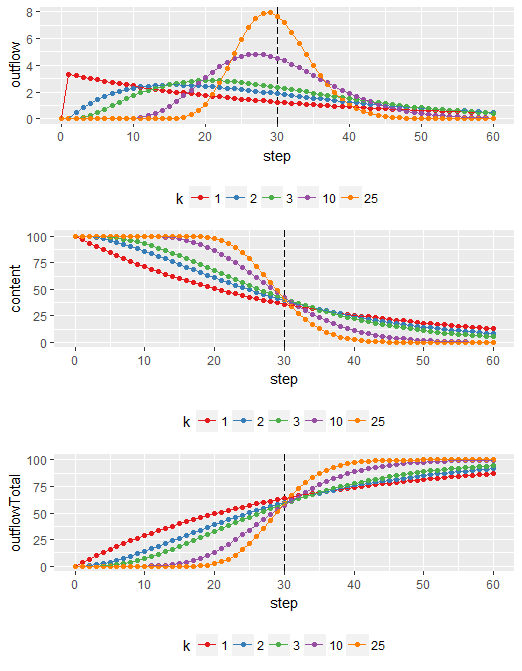
\includegraphics[width=.9\textwidth]{graphics/phys-dev-1}
\caption{Three commonly used outputs from the \code{Stage} class: \code{outflow}, \code{content} and \code{outflowTotal}. Stage inputs \code{duration} set to 30 and \code{k} set to different values. Produced by the \filename{\inputfolder/book/phys-dev-1.box} script.}
\label{fig:phys-dev-1}
\end{figure}


Rarely will all the inflow to a \code{Stage} box come as one initial pulse as shown in \iref{fig:phys-dev-1}. Usually, some amount will enter the box in every time step. The amount of inflow entering a \code{Stage} box a any time during a simulation is set by the \code{inflow} port. Since \code{inflow} is likely to vary dynamically, so will \code{outflow} and \code{content}.

\citet{Vansick77} extended the distributed delay with a parameter that he called 'attrition'; he was considering the loss of material during the distributed delay. However, his parameter can be used to model growth during the delay as well, so we call this input port \code{growthFactor}. All material entering a \code{Stage} box will appear later scaled by \code{growthFactor}. Its default value is 1. The \filename{book/phys-dev-2.box} script shows the effect of \code{growthFactor} (\iref{fig:phys-dev-2}). Here it has been held at three different, constant values but in a simulation model, \code{growthFactor} might as well be dynamic. It can be seen in the figure's bottom panel, that the initial 100 units emerge as 20, 100 or 200 units corresponding to \code{growthFactor} equal to 0.2, 1 or 2.

\begin{figure} [ht]
\centering
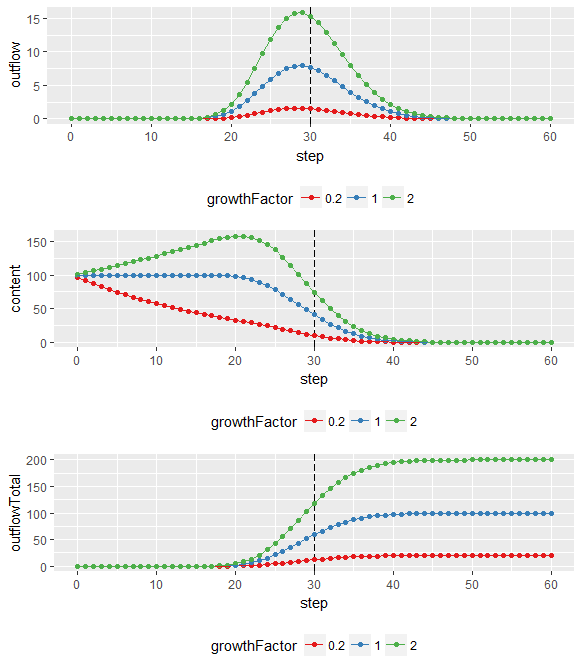
\includegraphics[width=.9\textwidth]{graphics/phys-dev-2}
\caption{Three commonly used outputs from the \code{Stage} class: \code{outflow}, \code{content} and \code{outflowTotal}. Stage inputs \code{duration} set to 30 and \code{growthFactor} set to different values. Produced by the \filename{\inputfolder/book/phys-dev-2.box} script.}
\label{fig:phys-dev-2}
\end{figure}

With $\code{growthFactor}<1$ you can model a loss intrinsic to the process (the red curves in \iref{fig:phys-dev-2}); the \code{growthFactor} proportion of the inflow will quietly seep away. If you want to model sudden death to a \code{Stage} box, you must use the \code{instantLossRate} port instead of \code{growthFactor}. It's common to confuse these two inputs although they work very diffently.

The default value of \code{instantLossRate} is zero, and that is likely how you want to keep it most of the time, if you want anything left alive in your simulation. If $\code{instantLossRate}>0$ then the proportion $\code{instantLossRate}$ of the content of the \code{Stage} box will be lost immediately. This is useful for modelling, for example, predation and acute toxic events. In \iref{fig:phys-dev-3} you can see, how two events of $\code{instantLossRate}>0$ plays out.

\begin{figure} [ht]
\centering
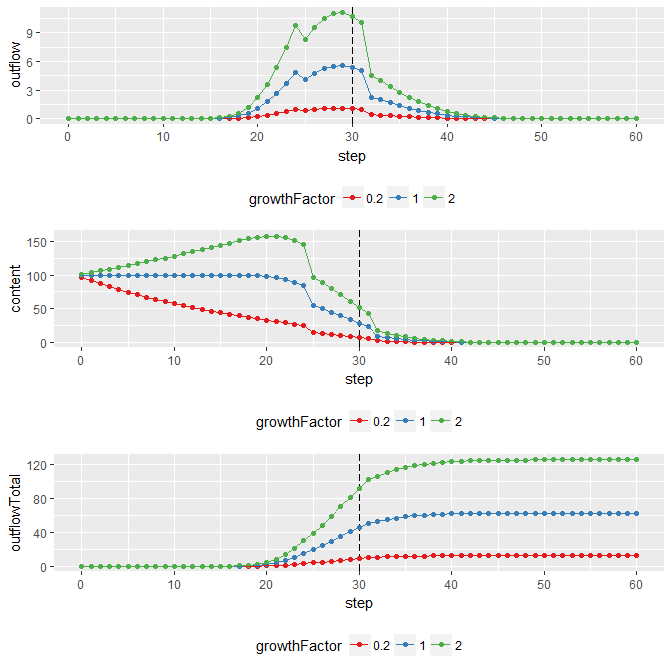
\includegraphics[width=.9\textwidth]{graphics/phys-dev-3}
\caption{Outputs as in \iref{fig:phys-dev-2}, except for \code{instantLossRate} set to 0.3 in step 25 and 0.5 in step 32. Produced by the \filename{\inputfolder/book/phys-dev-3.box} script.}
\label{fig:phys-dev-3}
\end{figure}

You may wonder if it wouldn't be usefull with a parameter for instant growth as well, \ie\ a factor by which the content is immediately scaled up, rather than reduced? However, experience has taught me that this is a problematic method to model growth with the distributed delay. How to model growth is further discussed in \iref{ch:devappl}.

Internally, a \code{Stage} box keeps track of its content as $k$ cohorts kept in a vector. The \code{content} port simply gives you the current sum of the cohort vector. When the \code{Stage} box is updated, the whole cohort vector is scaled by $(1-\code{instantLossRate})$. 

In some models, you may want to take away a proportional slice of the cohorts and use it as input for some other box. This is achieved by setting  \code{phaseOutflowProportion} $>0$. The slice of the cohort vector lost is available through the \code{phaseOutflow} port (\iref{fig:phys-dev-stage}). Mirroring this, a slice can be added (as a vector of the same length as the cohort vector) through the \code{phaseInflow} port. 

The two ports \code{instantLossRate} and \code{phaseOutflowProportion} both take away a proportion of the cohort vector. However, the former is applied before stage development is effectuated, \ie before \code{inflow} is added and \code{outflow} is calculated (\iref{fig:phys-dev-stage}), while the latter is applied after stage development. Practical experience with \code{Stage} has led to this slight difference in computation order. It also allows you to apply both at the same time, \ie\ $\code{instantLossRate}>0$ and $\code{phaseOutflowProportion}>0$

\begin{figure} [ht]
\centering
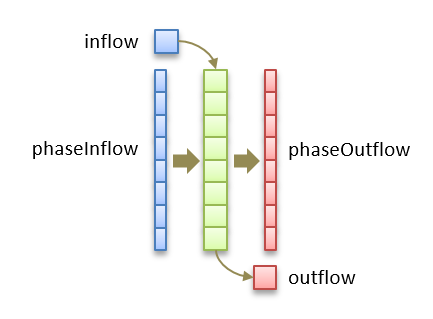
\includegraphics[width=.5\textwidth]{graphics/phys-dev-stage}
\caption{The flows in and out of a \code{Stage} box.}
\label{fig:phys-dev-stage}
\end{figure}

The two ports, \code{phaseInflow} and \code{phaseOutflow}, allow a crosscurrent through a \code{Stage} box. In your mind's eye, you should imagine material flowing vertically as passing through a \concept{stage}, and material flowing laterally passing through a \concept{phase}. These two concepts were chosen to distinguish between simultaneous, orthogonal development processes. How this can be usesul will be more evident, when we next consider bi-directional development.

\FloatBarrier
\section{Bi-directional development (\code{StageAndPhase})}

If we re-consider the design of the \code{Stage} class (\iref{fig:phys-dev-stage}), it is unsatisfying that the vertical and lateral flows work on different principles. Could we reconcile this difference? The two-dimensional distributed delay of \citet{Larkin00} comes to rescue (\iref{fig:phys-dev-stage-2d}).

\begin{figure} [ht]
\centering
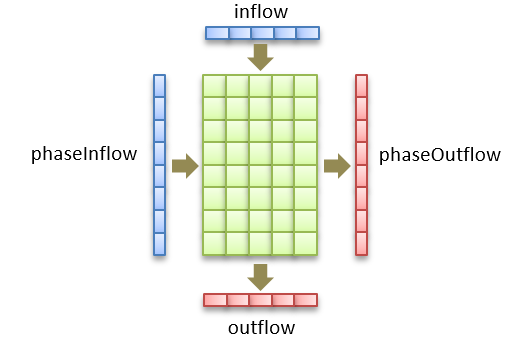
\includegraphics[width=.5\textwidth]{graphics/phys-dev-stage-2d}
\caption{The flows in and out of a \code{StageAndPhase} box.}
\label{fig:phys-dev-stage-2d}
\end{figure}

\begin{figure} [ht]
\centering
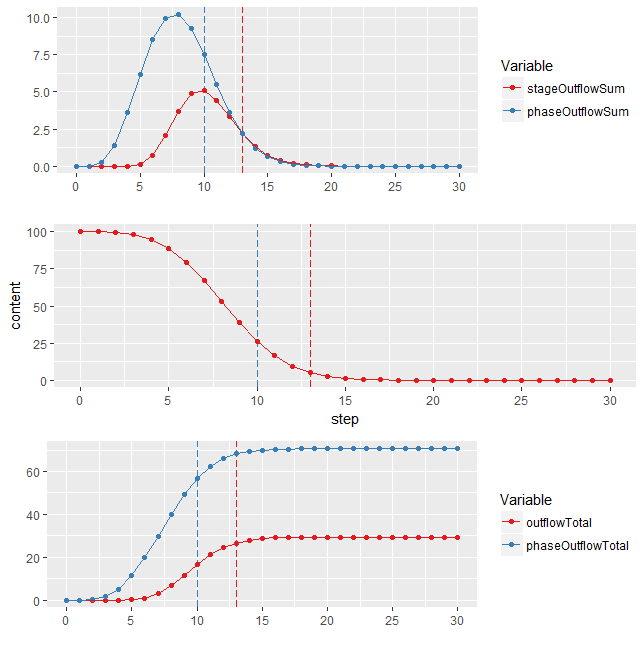
\includegraphics[width=.9\textwidth]{graphics/phys-dev-4}
\caption{Outputs from a \code{StageAndPhase} box with stage parameters, \code{duration} = 13 (red-dashed line) and \code{k} = 10, and phase parameters, \code{phaseDuration} = 10 (blue-dashed line) and \code{phaseK} = 5. Produced by the \filename{\inputfolder/book/phys-dev-4.box} script.} 
\label{fig:phys-dev-4}
\end{figure}

In this model, cohorts are kept in a matrix to represent ageing along two dimensions. All flows into and out of the box are represented as vectors. Compare that with the \code{Stage} class, in which vertical flows are scalars and lateral flows are vectors (\iref{fig:phys-dev-stage}).
 
The \code{StageAndPhase} class is equipped with inputs for  lateral (phase) development (\code{phaseK}, \code{phaseDuration} and \code{phaseTimeStep}), together with inputs for vertical (stage) development (\code{k}, \code{duration} and \code{timeStep}).
 
An example of \code{StageAndPhase} outputs is seen in \iref{fig:phys-dev-4} which replicates Fig. 5 in \citet{Larkin00}. For a \code{StageAndPhase} box the \code{initial} input is still a scalar (100, in this example). At time zero it is placed in the upper left corner of the cohort matrix. When comparing the figures, it seems that the \code{StageAndPhase} implementation leads material through a bit faster than the Larkin at al. implementation. The reason for this slight discrepancy has not been investigated.  

The initial 100 units change phase faster than stage (mean duration of 10 \vs\ 13) and with a larger dispersion ($k$ equal to 5 \vs\ 10) (\iref{fig:phys-dev-4}). Hence, in the end, more material has changed phase (70.6) than stage (29.4) (the precise numbers were looked up in the \code{sim} data frame in R). 

\begin{figure} [ht]
\centering
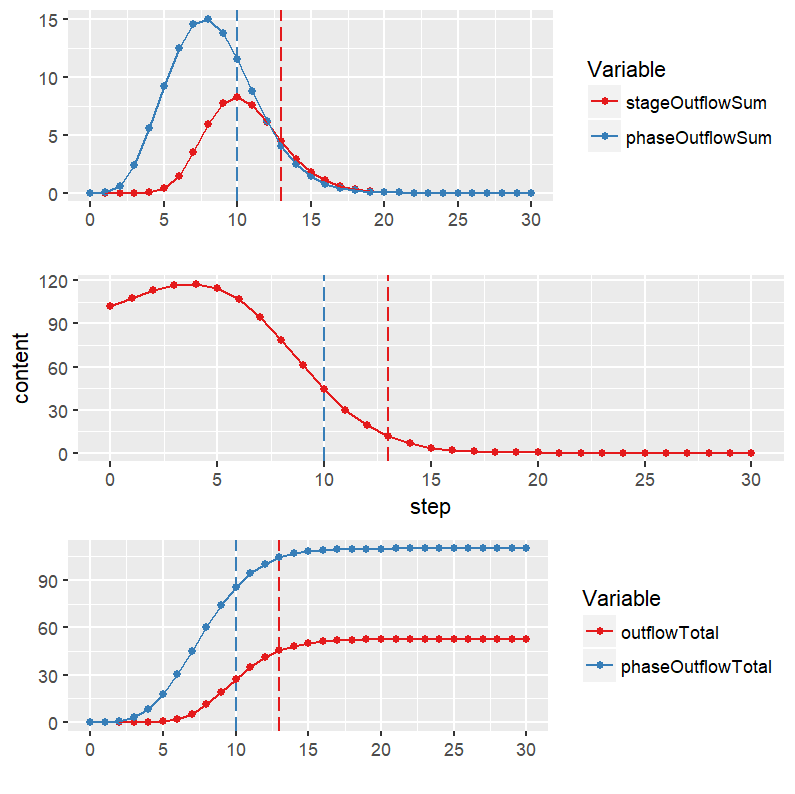
\includegraphics[width=.9\textwidth]{graphics/phys-dev-5}
\caption{Outputs from a \code{StageAndPhase} box as in \iref{fig:phys-dev-4}, except with \code{growthFactor} = 2. Produced by the \filename{\inputfolder/book/phys-dev-5.box} script.} 
\label{fig:phys-dev-5}
\end{figure}

However, note that both outflows are faster than their nominal means, indicated by the vertical lines (\iref{fig:phys-dev-4}). Each flow on its own would obey its mean delay but running together, the two processes drain the content faster leading to an overall faster drain of the box. One should be aware of this effect when estimating parameters for the two-dimensional distributed delay.
 
What happens if we set $\code{growthFactor} > 1$ for a \code{StageAndPhase} box? The outcome of this experiment (\iref{fig:phys-dev-4}) is discouraging. The timing and shape of the outflows seem unchanged compared to the simulation without growth (\iref{fig:phys-dev-5}). However, the stage (52.5) and phase (109.9) outflows only add up to 162.4 which is less than the expected 200, with a \code{growthFactor} = 2 working on an initial 100 units.

The math of the two-dimensional distributed delay has not yet been worked out. There is no equation that tells us the effective mean and variance of the stage and phase outflows, resulting from the set mean durations and $k$ values. Likewise, it has not been worked out how to apply a growth factor during the delay to achieve a desired scaling of the input to outputs. 

Due to its complexity the \code{StageAndPhase} model should be used only when the simpler \code{Stage} model cannot provide the needed functionality. One such case, is in epidemiological modelling which is one of the applications treated next.

\FloatBarrier
\section{Applications}
\label{ch:devappl}
\subsection{Phenology and population dynamics}
In its simplest application, a series of \code{Stage} boxes can be linked, \code{outflow} to \code{inflow}, to represent the phenology of development through a sequence of life stages (\iref{fig:phys-dev-appl-1}). A final \code{Stage} box simulates reproduction, working in parallel with the \code{Stage} box for adult development. Thus both phenology and population dynamics can be modelled by the application of \code{Stage} boxes.

\begin{figure} [ht]
\centering
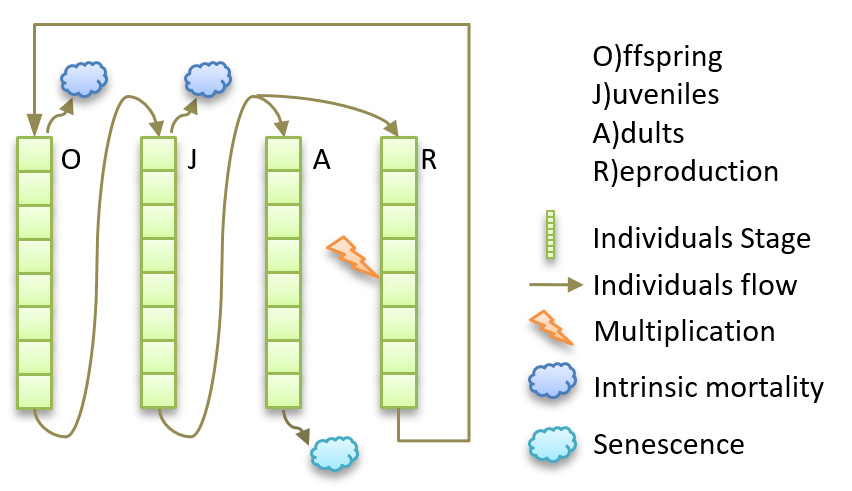
\includegraphics[width=.9\textwidth]{graphics/phys-dev-appl-1}
\caption{Three \code{Stage} boxes in sequence representing life stages plus one \code{Stage} box for reproduction}. 
\label{fig:phys-dev-appl-1}
\end{figure}

Each \code{Stage} box contains the number of individuals in that stage. Through \code{growthFactor} < 1 the intrinsic mortality of immature stages can be included (for offspring and juveniles in \iref{fig:phys-dev-appl-1}), while mortality of the last, usually adult, stage occurs through the stage \code{outflow} leading nowhere.

Reproduction is modelled by leading juvenile \code{outflow} to both the adult and reproduction boxes in parallel (\iref{fig:phys-dev-appl-1}). Through \code{growthFactor} > 1 the reproduction box will mimic multiplication of adults into reproductive output, corresponding to the net reproductive rate of the population. The reproduction \code{outflow} is led back to the offspring where it enter as \code{inflow}.

If \code{growthFactor} for the reproduction box is fixed, the model will lead to unlimited growth---exponential, as soon as the stage-distribution has stabilised. A more realistic model would include density-dependent boxes supplying survival rates, which could be used to reduce the stage-specific \code{growthFactor} inputs. Remember, that \code{growthFactor} is not a rate per time unit, \eg\ per day or day-degree, but applies to the whole box, scaling input to output during development.

It is not shown in \iref{fig:phys-dev-appl-1}, how the population is initialised. Depending on the biology of the species and the ecological setting, individuals could enter  any life stage as an \code{inflow} to represent immigration or individuals breaking diapause. Separate boxes, with logic driven by \eg\ weather and calendar, would be needed to compute these intermittent inflows.

\subsection {Number and mass dynamics}

Population numbers (\ie number of individuals) and mass can be modelled by running two separate sequences of \code{Stage} boxes
in parallel (\iref{fig:phys-dev-appl-2}).

\begin{figure} [ht]
\centering
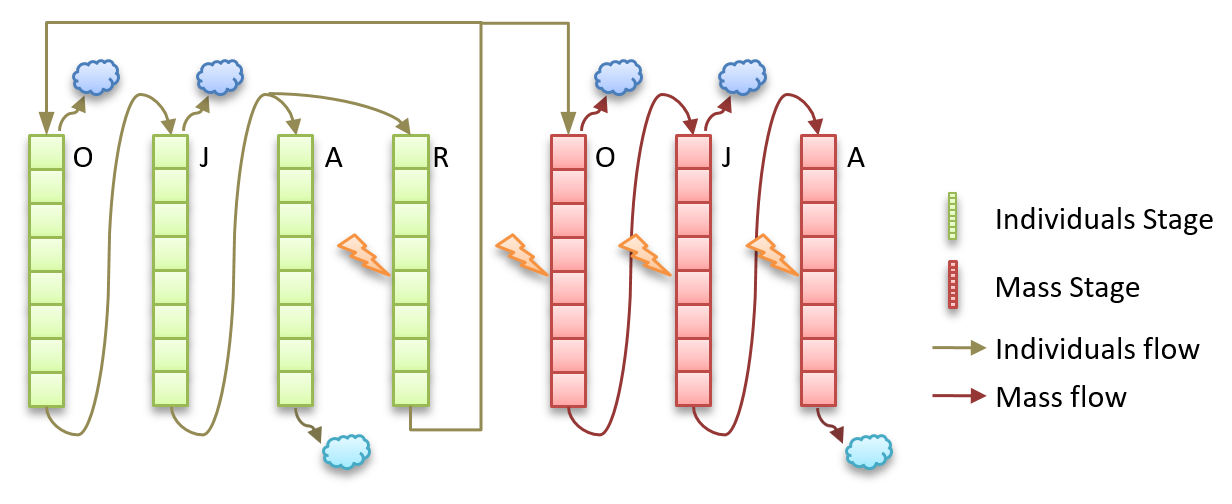
\includegraphics[width=.9\textwidth]{graphics/phys-dev-appl-2}
\caption{Two sequences of \code{Stage} boxes running in parallel to represent population numbers and mass. Notation as in \iref{fig:phys-dev-appl-1}, except as noted.} 
\label{fig:phys-dev-appl-2}
\end{figure}

Mass increases while passing through the mass \code{Stage} boxes by setting \code{growthFactor} > 1. Logically, there is no need for a reproduction box among the mass boxes parallel to the number reproduction box. The intrinsic mortality for juvenile stages applies equally to number and mass boxes; however, for the mass boxes, the rate of somatic growth must be factored in.

This method of modelling somatic growth will, however, work smoothly only in the simple cases when growth is fixed. Remember, once again, that \code{growthFactor} will be applied over the the whole duration of the stage. A \code{growthFactor} of 50, for example, would mean that for \SI{1}{\gram} entering \SI{50}{\gram} would eventually exit. If this is true only when the ressources, on which the population depends, are assumed limitless, how would one take realistic variation of the resources into account?
 
A \code{Stage} box has an output \code{growth} which tells how much growth there was during the last time step (\iref{fig:phys-dev-6} bottom). In the example shown, the \code{Stage} box  undergoes a multiplication by 2 during development, starting from an initial 100 units. Let's assume this box models mass growth, \ie\ it goes from \SI{100}{\gram} to \SI{200}{\gram}.

 \begin{figure} [ht]
\centering
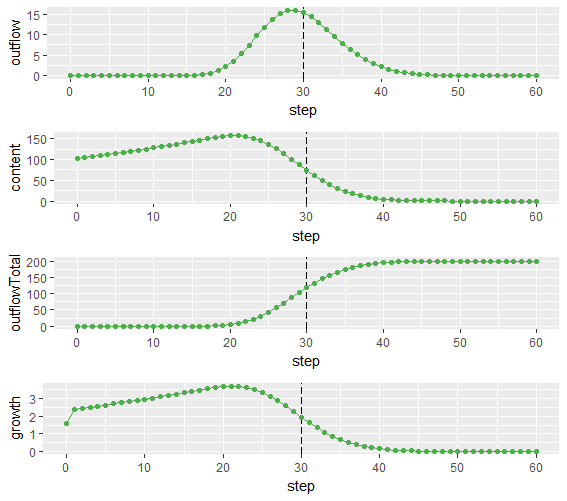
\includegraphics[width=.9\textwidth]{graphics/phys-dev-6}
\caption{Simulation outputs from a \code{Stage} box with \code{growthFactor} = 2, as also seen in \iref{fig:phys-dev-2}. Produced by the \filename{\inputfolder/book/phys-dev-6.box} script.} 
\label{fig:phys-dev-6}
\end{figure}

It can be seen (\iref{fig:phys-dev-6}) that growth is around \SI{3}{\gram} per time step during most of the development time, decreasing towards the end. This is actually the growth demand of the population represented by this box. Depending on its energy budget (\iref{ch:trophic-energy-budget}) this would translate into a certain resource demand, which would  be acquired through a functional response model (\iref{ch:trophic-functional-response}).

It is not straightforward to include varying supply/demand ratios in a model with mass dynamics. The exact implementation will depend on the physiology of the organism.

\subsection {Predator-prey and parasitoid-host}
In a predator-prey model, predator and prey can both be represented as a sequence of life stages held in \code{Stage} boxes, which contain the number of individuals in each life stage (\iref{fig:phys-dev-appl-3}). 

The reproductive outflow of the predator is not transfered directly into the offspring box. Instead, it is interpreted as the predator's demand for offspring production. Thus it enters the functional response (\iref{ch:trophic-functional-response}) and energy budget model (\iref{ch:trophic-energy-budget}), the outcome of which is, on one side, the number of prey killed, on the other side, the number of predator offspring produced. The energy budget translates prey killed into predator offspring. See \iref{ch:trophics-predator-prey-energy-budget} for a working model.

In this example, only one prey life stage is attacked by the predator. In other cases, more than one life stage may be attacked, with different attack rates and different exchange rates of prey into predator offspring. This can be sorted out as a food web (\iref{ch:trophics-food-web}).

If we consider this instead a parasitoid-host system, we find that, structurally, there a no differences. The outflow from the predator's reproduction box is then a demand for egg-laying, which is turned into a realised egg-laying rate by the functional response. For most parasitoids, there is a one-to-one relationship between the number of hosts parasitised and the number of eggs laid, which makes the exchange rate simply 1:1. A working model can be found in \iref{ch:trophics-parasitoid-host}.

\begin{figure} [ht]
\centering
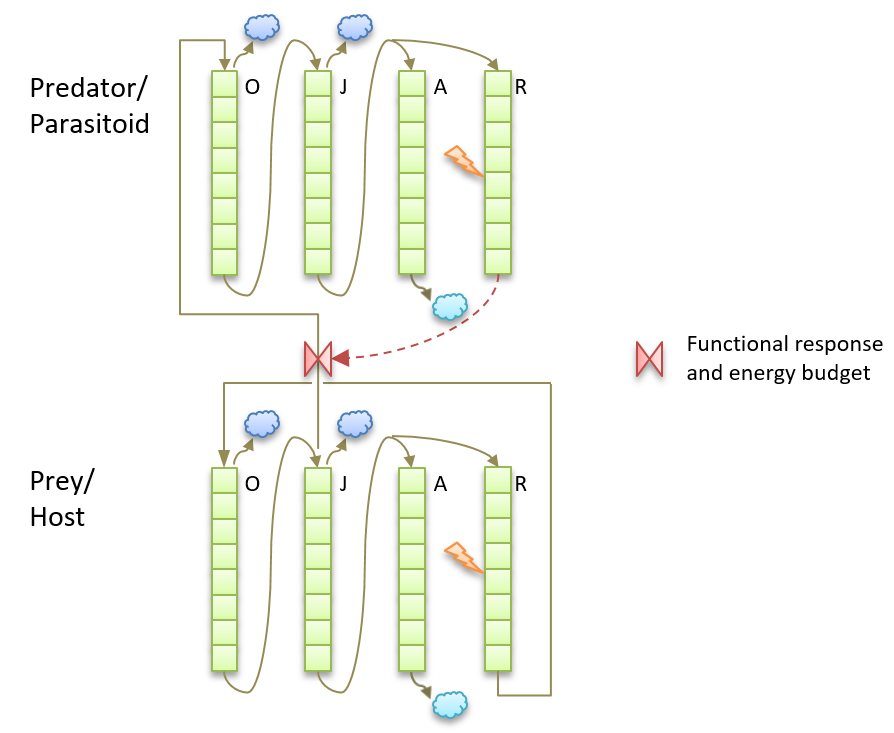
\includegraphics[width=.9\textwidth]{graphics/phys-dev-appl-3}
\caption{Predator (or parasitoid) and prey (or host) sequences of \code{Stage} boxes connected by predator functional response and energy budget. Notation as in \iref{fig:phys-dev-appl-1}, except as noted.}
\label{fig:phys-dev-appl-3}
\end{figure}

\subsection {Insect pathogen}

In this example, an insect pathogen is modelled in terms of a population of cadavers which develops into a population of spores (\iref{fig:phys-dev-appl-4}). In the cadaver stage the pathogen undergoes multiplication. In the spore stage, the spores remain infectious until they degrade and exit as \code{outflow} from the spore \code{Stage} box. 

The current number of infectious spores (accessed through the \code{content} port of the \code{Stage} class) feeds into a functional response model (\iref{ch:trophic-functional-response}), which determines how many hosts get infected and  transferred to the cadaver box. Compare this with the previous example (\iref{fig:phys-dev-appl-3}), where it was the \code{outflow} of the reproductive stage that fed information into the functional response.

The exchange rate (energy budget) of this interaction could simply be 1:1, as one host turns into one cadaver. If more than one host stage is infected, the exchange rate might need to differ between hosts, \eg\ if a smaller host would provide less material for spore production than a larger host.

\begin{figure} [ht]
\centering
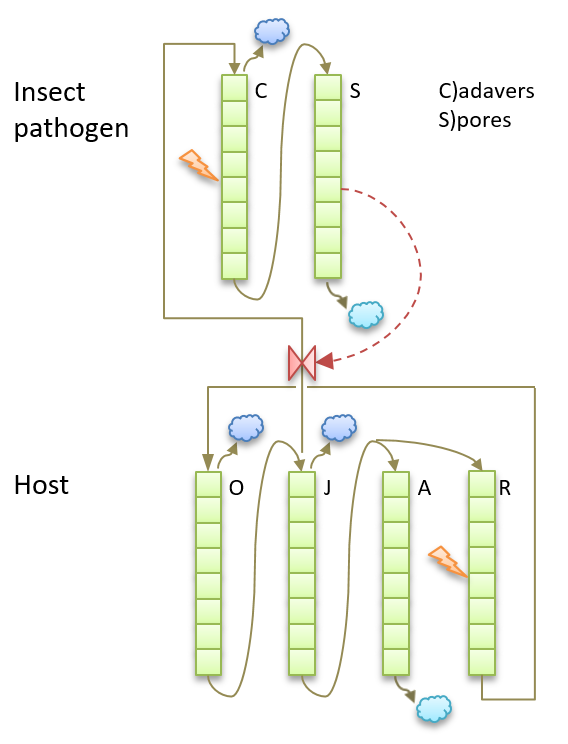
\includegraphics[width=.6\textwidth]{graphics/phys-dev-appl-4}
\caption{The cadaver and spore stages of an insect pathogen connected by a functional response to a host population. Notation as in \iref{fig:phys-dev-appl-3}, except as noted.} 
\label{fig:phys-dev-appl-4}
\end{figure}

%
% \subsection {Epidemiology (SEIR)}
% The modelling of epidemics in humans and animals has a long history which has crystalised in the common framework of SEIR models \citep{KeeRoh08}. This acronym stands for the phases of infection a host might go through: susceptible, exposed, infectious and resistant. For any specific system, one or more phases may apply.

% Before we combine the  \concept{stage} changes of host development with the \concept{phase} changes  of an infection, let us take a look at the succession of phase changes in isolation. Consider a population going through the SEIR phases (\iref{fig:phys-dev-appl-5}). The S stage is simply a \code{Stage} box. The individuals develop through this stage, entering young at the top and leaving it senescent at the bottom. Meanwhile they grow as shown by the multiplication symbol in the figure.

% \begin{figure} [ht]
% \centering
% 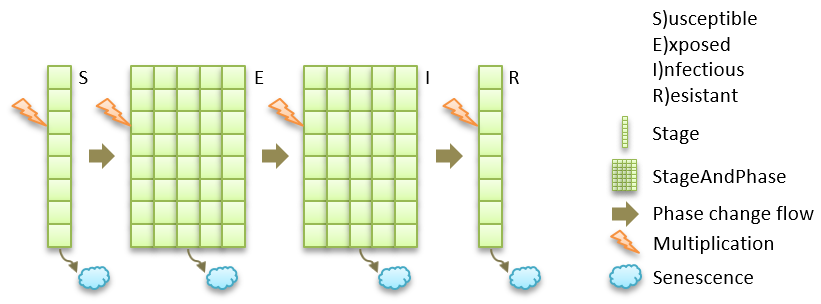
\includegraphics[width=.9\textwidth]{graphics/phys-dev-appl-5}
% \caption{An epidemiological model of a population going through the four SEIR phases.} 
% \label{fig:phys-dev-appl-5}
% \end{figure}

% Due to mechanisms not accounted for in this model, a proportion of the S individuals becomes exposed in every simulation time step and enter the E box which is of the \code{StageAndPhase} class. Here the individuals continue their development (vertically) as before but at the same time undergo phase change (laterally) according to the pace of the infection's progress.

% Senescent indiduals leave the E box at the bottom but now as a cohort (a row vector) of individuals, according to how far they got through the E phase  (laterally) before dying. Individuals, when completing the E phase, leave as a cohort (a column vector) of individuals to enter the I phase. This cohort reflects how far the individuals got through ageing (vertically) before changing phase.

% The I box works just lihe the E box while for the final R phase, we are back to a simple \code{Stage} box. At this point, phase change is no longer possible (at least in this model).

% The model in \iref{fig:phys-dev-appl-5} was implemented in the \filename{\inputfolder/book/phys-dev-appl-5.box} script. You can load it and type \code{list} at the \US\ prompt to get an overview of the many boxes.

% The model starts with an \code{initial} 10 individuals in the S box. For the lateral flows to match, the dimension (\code{k}) of the development cohorts (column vectors) must be the same for all four boxes (). In this example, it was chosen to set \code{k}=25, \code{duration}=13 and \code{growthFactor}=30 for all four boxes. 

% The E and I boxes do not need to have the same values for phase change. Here we set \code{phaseK}=5 and \code{phaseDuration}=10 for the E box, and \code{phaseK}=6 and \code{phaseDuration}=15 for the I box.

% The output from the simulation (\iref{fig:phys-dev-appl-5-output}) shows, as expected, that senescent individuals leave the system in the order SEIR. Note that for the \code{Stage} boxes S and R, the \code{outflow} port is shown, whereas for the \code{StageAndPhase} boxes E and I, the \code{stageOutflowSum} port is shown. The latter provides the sum of the outflow, leaving in every time step as a row vector.

% The total, accumulated outflows as reported at the R prompt are S=158.1, E=95.8, I=38.1 and R=8.1. The sum of these amounts to 300, as expected given the initial number (10) and the common growth factor (30) for all four boxes.

% \begin{figure} [th]
% \centering
% 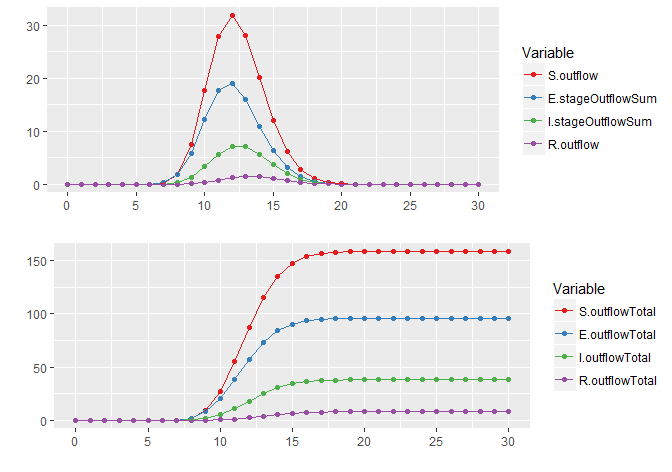
\includegraphics[width=.9\textwidth]{graphics/phys-dev-appl-5-output}
% \caption{A simulation of the system shown in \iref{fig:phys-dev-appl-5}. Produced by the \filename{\inputfolder/book/phys-dev-appl-5.box} script. } 
% \label{fig:phys-dev-appl-5-output}
% \end{figure}

% Next, let's look at a fully fledged SEIR model involving a host and a vector-born disease (\iref{fig:phys-dev-appl-6}) implemented in the \filename{\inputfolder/book/phys-appl-6.box} script. \concept{The host population} is divided into two stages: juvenile and adult. 

% The disease is not vertically (\ie\ maternally) transmitted. Hence the host holds a reproduction box only for the susceptible stage (host R box in \iref{fig:phys-dev-appl-6}). This R box collects juvenile outflows from all four host phases and yields only susceptible eggs.

% Exposure happens at a rate that depends on the density of infectious vector adults (think of the vector as a mosquito). However, to keep this model simple, the exposure rates for juveniles and adults (arrows $e$ and $l$ in the figure) were set to fixed proportions, \SI{0.04}{\per\day} and \SI{0.01}{\per\day}, of the juvenile and adult contents, respectively. 

% All phase changes (S$\rightarrow$E, E$\rightarrow$I and I$\rightarrow$R) are effectuated for both the juvenile and adult boxes. Whereas the phase change from S to E depends on the interaction with vector adults, the two subsequent phase changes are driven by the intrinsic rates of phase change. Thus the average duration of phases E and I were set to \SI{10}{\day} and \SI{20}{\day}, respectively. The duration of the juvenile and adult stages were set to the same for all SEIR phases, \SI{10}{\day} and \SI{30}{\day}, respectively.

% \begin{figure} [h!]
% \centering
% 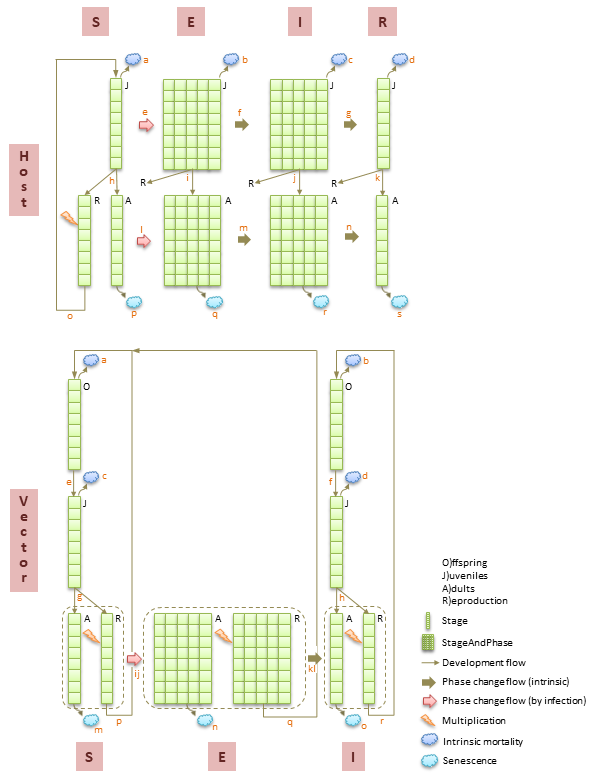
\includegraphics[width=\textwidth]{graphics/phys-dev-appl-6}
% \caption{An SEIR model involving a host and a vector population both stage-structured. Lowercase letters $a$ to $s$ for the host and $a$ to $r$ for the vector refer to explanations in the text.} 
% \label{fig:phys-dev-appl-6}
% \end{figure}

% Individuals leave the model by intrinsic mortality in the juvenile stages (clouds marked $a$ to $d$), although this was set to zero in this model (\ie\ \code{growthFactor}=1 for all \code{Stage} and \code{StageAndPhase} boxes). Otherwise, individuals die from senescence as they leave the adult stages (clouds marked $p$ to $s$).

% \concept{The vector population} is divided into three stages: offspring, juvenile and adult. A box for reproduction follows the box of adult individials through the three phases SEI. The exposure of adult and reproduction boxes (arrow denoted $i$ and $j$ for the two lateral flows) depends on the density of infectious juvenile and adult hosts, but for simplicity in this model is kept at a constant rate as a proportion (\SI{0.04}{\per\day}) of the adult and reproduction boxes, respectively.

% As for the host model, intrinsic mortality (clouds marked $a$ to $d$) was set to zero throughout. Senescent individuals leave as clouds marked $m$ to $o$. Reproductive output from the S and E phases (arrows $p$ and $q$) are both led to offspring of the S phase, while infectious mothers are assumed to produce 100\% infectious eggs (arrow $r$). A more realistic model would maybe split the reproductive output from the I phase ($r$) between S and I offspring.

% To be able to verify that this meshwork of flows and boxes works as intended, the first implementation of the model in the \filename{\inputfolder/book/phys-dev-appl-6.box} script was configured with zero reproduction. This allows us to follow the fate of the initial populations through stage developments and phase changes. The initial numbers were 80 juvenile and 50 adult S hosts, together with 100 offspring of S vectors. Remember too that the host and vector populations do not interact in this model, as all exposure rates (red arrows) were set to fixed rates in proportion to the S box contents.

% The population dynamics (\iref{fig:phys-dev-appl-6-output}) show how the juvenile hosts (top panel) go through a succession of SEIR phases, although none seem to reach the R phase. A similar pattern is seen for the adult hosts (next panel down) but due to their longer life span, discernable numbers reach the R phase.

% The output found at the R prompt (not shown here) attests that the total flow through $e$ and $h$ (\iref{fig:phys-dev-appl-6}) amounts to the initial number of juvenile hosts (80). Moreover the total output of scenescent individuals ($p+q+r+s$) amounts to the sum of initial juveniles (80) and adults (50), \ie\ a total of 130 individuals which die of old age. This was expected because no intrinsic mortality ($a$ to $d$) was included in the model. Finally, total reproduction (arrow $o$) was as expected with a host fecundity of 2.5, $o=2.5\times(80+50)=325$.

% The adult vector population likewise goes through a succession of phases: SEI (\iref{fig:phys-dev-appl-6-output} bottom panel). The reproductive output is spread over all three phases and sums up to the expected total, given the initial population size (100) and fecundity (5): $p+q+r=287.9+37.7+174.4=500$. The initial 100 offspring survives unscathed until dying of old age: $m+n+o=57.6+6.8+35.6=100$.

% \begin{figure} [h!]
% \centering
% 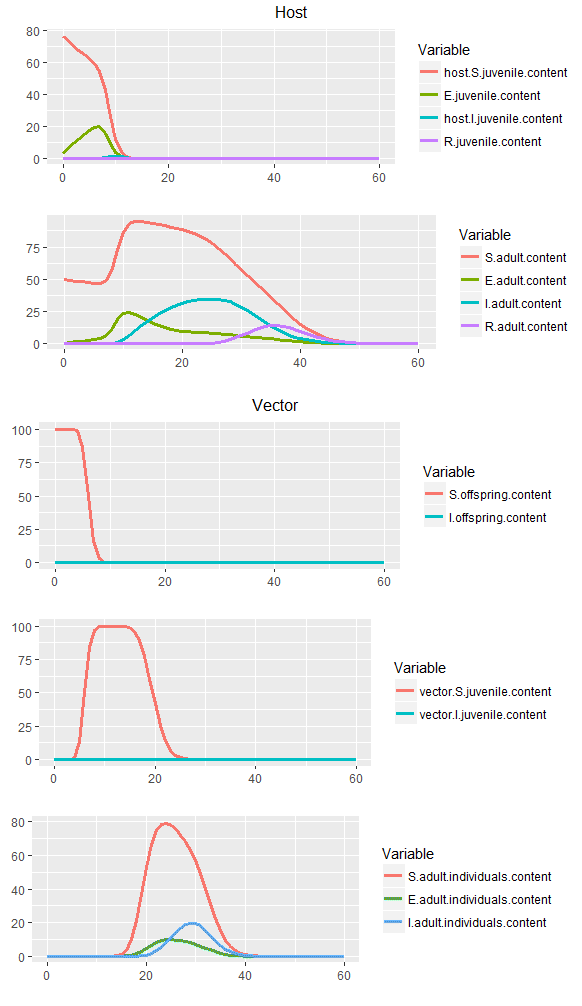
\includegraphics[width=.9\textwidth]{graphics/phys-dev-appl-6-output}
% \caption{Dynamics of the SEIR model in \iref{fig:phys-dev-appl-6} \emph{without} reproduction. Produced by the \filename{\inputfolder/book/phys-dev-appl-6.box} script.} 
% \label{fig:phys-dev-appl-6-output}
% \end{figure}

% \begin{figure} [h!]
% \centering
% 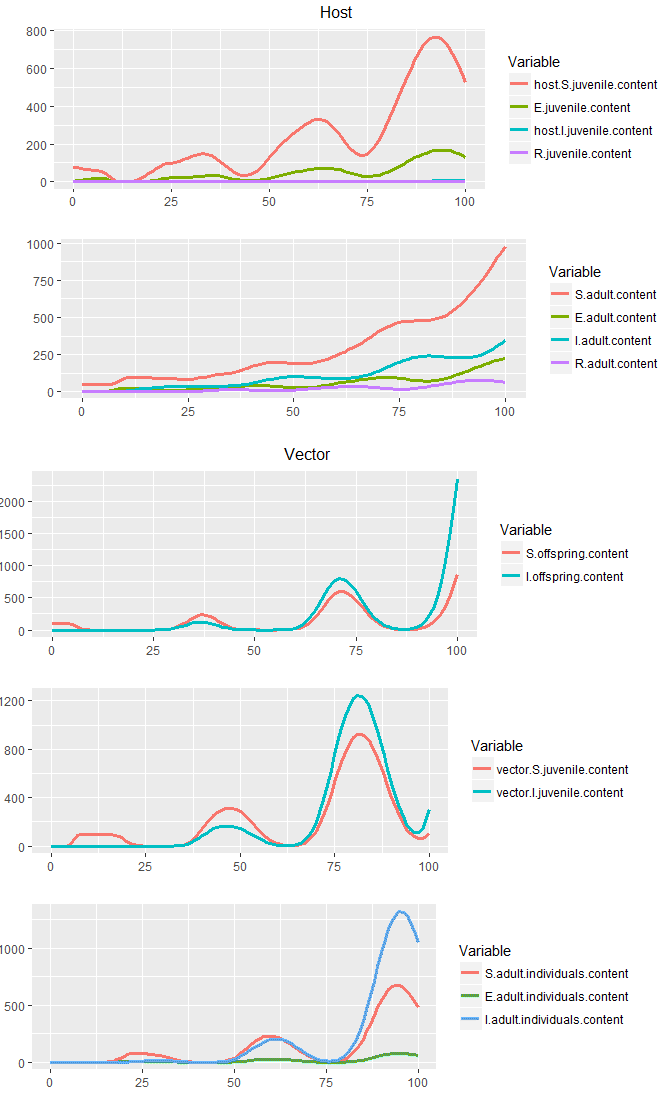
\includegraphics[width=.9\textwidth]{graphics/phys-dev-appl-7-output}
% \caption{Dynamics of the SEIR model in \iref{fig:phys-dev-appl-6} \emph{with} reproduction. Produced by the \filename{\inputfolder/book/phys-dev-appl-7.box} script.} 
% \label{fig:phys-dev-appl-7-output}
% \end{figure}

% \FloatBarrier
% Having verified that the wiring between boxes is correct, we can finally let the population dynamics loose. In the \filename{\inputfolder/book/phys-dev-appl-7.box} script, reproduction is effectuated for both host and vector. This results in increasing population densities with an underlying complexity of life stages and SEIR phases (\iref{fig:phys-dev-appl-7-output}).

% SEIR models are inherently complex. Even though the model presented is complex, it still misses to take the host-vector interactions into account (\ie\ the three red arrows in \iref{fig:phys-dev-appl-6}). You should build SEIR models (and any other models) piecewise and along the way verify that they work properly. The model presented here was not built in one swoop, nor was it built without errors on the way. It did not even turn out as it was first drafted on paper. There are so many biological mechanisms and interactions on which you must make up your mind in a host-vector model, that the model becomes an important thinking tool. Your understanding of the real-world system will grow as you develop the model. Even for SEIR models that do no involve a vector but instead a contagious disease, biological complexity may creep in on you. Whatever you do: Make sure what your assumptions are --- and that they make biological sense!

% % More complications could be added to this model. Foremost, you would need to model the exposure rates (the three red arrows in \iref{fig:phys-dev-appl-6}) to take the host-vector interactions into account. Most easily (and most correctly; yes, sometimes it is easier to do the correct thing) you can model these interactions using a \code{FoodWeb} box (see \iref{ch:trophicmultiple}). If the vector is a mosquito, its demand will be defined by a number of blood meals per female per day. Its attack rate should be defined for all three vector populations (adult vectors in all SEI phases) on all eight host populations (juvenile and adult hosts in all SEIR phases). Possibly the attack rate on juvenile hosts would be larger than on adult hosts. Furthermore, infectious vectors might have an altered  behaviour (an increased demand would make sense from the disease agent's point of view). This $3 \times 8$ attack matrix will result in 24 supply rates (sorted out by the \code{FoodWeb} box). It will be up to you to figure out how these supply rates should be effectuated. Obviously, some will translate into exposure rates. For a mosquito vector, the fecundity would depend on its supply of blood meals.

%
\section{Time scales}
The \code{Stage} class has a \code{timeStep} input port which defaults to 1. This means that for every simulation step, time progresses 1 unit by default for a \code{Stage} box. This must be interpreted in the context of another \code{Stage} input which is \code{duration}. If you set $\code{duration}=28$ and keep the default $\code{timeStep}=1$ then the average duration of that box will be 28 simulation steps. 

Mostly you'll want to operate with some concrete time unit, like days. If so, you should also include a \code{Calendar} box in your box script. The default setting of a \code{Calendar} box sets the pace of time to 1 day, \ie\ for every simulation step the \code{Calendar} box is updated by 1 day. In effect, the \code{date} output of \code{Calendar} is updated by 1 day. It is now implicit that your \code{Stage} box with $\code{duration}=28$ and $\code{timeStep}=1$ specifies an average duration of 4 weeks.

\subsection{Linear scale: day-degrees}
For poikilothermic organisms, a temperature-dependent time scale is the norm in simulation models. The most basic one works in day-degrees and is implemented in the \code{DayDegrees} class. We can see how this works with the typical data shown in \iref{tab:phys-dev}.

\begin{table}[ht]
\centering
\caption{Development time ($L$) and rate ($1/L$) at different temperatures ($T$) for brown marmorated stink bug (\emph{Halyomorpha halys}). Data from \citet{Nielsen08}.}
\label{tab:phys-dev}
\begin{tabular}{rrr}
$T$ (\si{\celsius}) & $L$ (\si{\day}) & $1/L$ (\si{\per\day}) \\
\hline
15 & $\infty$ & 0.0000 \\
17 & 121.50   & 0.0082 \\
20 &  81.07   & 0.0123 \\
25 &  44.65   & 0.0224 \\
27 &  36.67   & 0.0273 \\
30 &  33.73   & 0.0296 \\
33 &  37.67   & 0.0265 \\
35 & $\infty$ & 0.0000 \\
\hline
\end{tabular}
\end{table}

If we depict the development rate as a function of temperature (\iref{fig:phys-dev-scale-1}), we see a clear linear relation above a lower threshold for development ($T_0$), until high temperatures work havoc upon the insect's physiology. The blue regression line was estimated for the five lower temperature measurements,

\begin{equation}
1/L=aT+b=0.00212T-0.0300 
\end{equation}
Note the units: $1/L$ (\si{\per\day}), $a$ (\si{\per\day\per\celsius}) and $b$ (\si{\per\day}). 

\begin{figure} [ht]
\centering
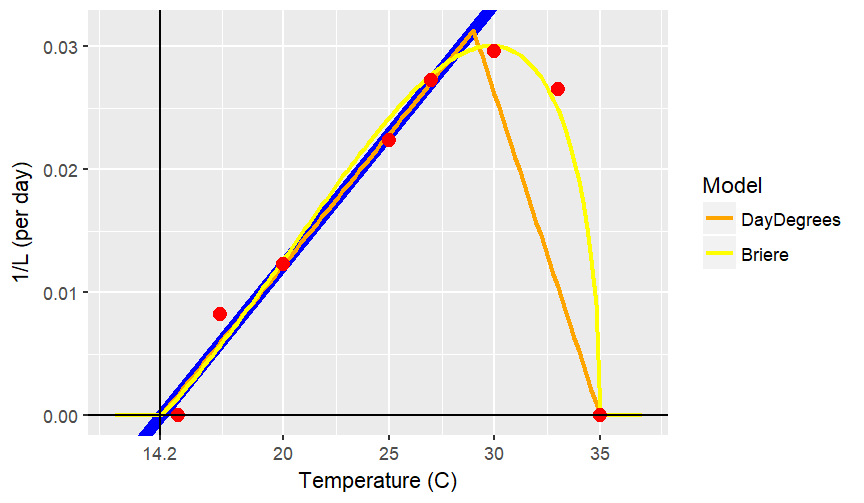
\includegraphics[width=.9\textwidth]{graphics/phys-dev-scale-1}
\caption{Observations from \iref{tab:phys-dev} (red dots) with regression line (blue), day-degree model (orange lines) and Briere model (yellow curve). Generated by the \filename{\inputfolder/book/phys-dev-scale.box} script.} 
\label{fig:phys-dev-scale-1}
\end{figure}

Think of $1/L$ running in  'proportional development per day'. This means, that if we for every day calculate $1/L$ from the regression line, according to the average temperature that day, and if we keep a tally accumulating these daily rates, then when this accumulation reaches 1, the insect has finished its development. This principle is called 'rate summation' and is basic to how you work with physiological time scales.

Since development rate will certainly not continue to increase with rising temperatures, the implementation in \code{DayDegrees} takes two inputs in addition to \code{T0}: \code{Topt} and \code{Tmax}, which sets the interval for a linear decrease in development rate at high temperatures. Thus we arrive at the two-segmented orange line in \iref{fig:phys-dev-scale-1}. This is how the \code{DayDegrees} model work, except for a final twist dictated by tradition.

Traditionally, the day-degree model is parameterised like this,

\begin{equation}
  1/L = \frac{T-T_0}{D_{sum}} \label{eq:day-degrees}
\end{equation}
with parameters easily derived from the linear regression above: $T_0=-b/a=-(-0.0300)/0.00212=\SI{14.2}{\celsius}$ and $D_{sum}=1/a=1/0.00212=\SI{472.1}{\day\celsius}$. The units \si{\day\celsius} are also known as day-degrees or degree-days. 

In summary, one would say about this insect that its average development time is 472.1 day-degrees above a lower threshold of \SI{14.2}{\celsius}. In the days before computers, this scale was convenient because the rate summation could be carried out more simply as a summation of daily temperatures above the lower threshold for development. Accordingly the \code{duration} input of a \code{DayDegrees} box specifies the average duration in day-degrees and its output \code{step} is the daily increment in day-degrees.

\subsection{Non-linear scales}
It is obvious from \iref{fig:phys-dev-scale-1} that, in this case, the day-degrees model does not handle high temperatures well, even with a breakpoint at the optimal temperature. For this reason it is tempting to use a non-linear scale which better summarises the observed development rates. The yellow curve (\iref{fig:phys-dev-scale-1}) is one such example, taken from \citet{Briere99}:

\begin{equation}
  1/L = aT(T-T_0)\sqrt{T_{max}-T} \label{eq:briere}
\end{equation}

An algebraic excursion will lead you to the (formidable looking) location of the optimum temperature:
\begin{equation}
T_{opt}= \frac{\sqrt{9T_0^2 - 16T_0T_{max} + 16T_{max}^2} + 3T_0 + 4T_{max}}{10} \label{eq:briere-opt}
\end{equation}

Maybe of more relevance is the finding, that if you want to define the curve by its optimum rather than its maximum temperature, you can calculate the maximum temperature from the optimal temperature:

\begin{equation}
T_{max} = \frac {T_{opt}(5T_{opt} - 3T_0)}{4T_{opt} - 2T_0}
\end{equation}


\begin{figure} [ht]
\centering
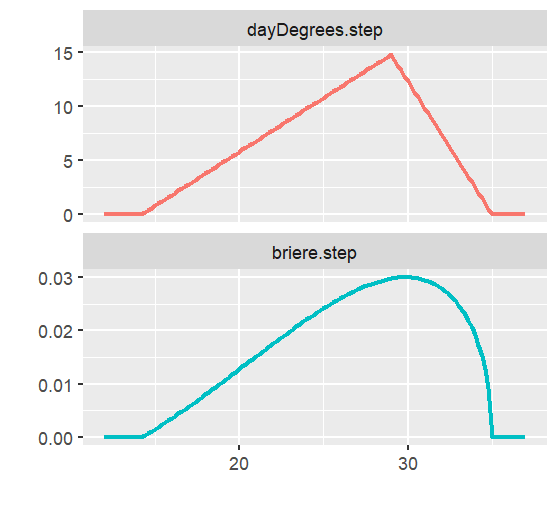
\includegraphics[width=.6\textwidth]{graphics/phys-dev-scale-2}
\caption{The \code{step} output calculated by a \code{DayDegrees} (top) and \code{Brieri} box (bottom) at different temperatures. Generated by the \filename{\inputfolder/book/phys-dev-scale.box} script.} 
\label{fig:phys-dev-scale-2}
\end{figure}

\Cref{eq:briere} is implemented in the \code{Briere} class. Its parameters were estimated from the data in \iref{tab:phys-dev} which resulted in the curve shown in \iref{fig:phys-dev-scale-1}. The \code{nls} function of R yielded these estimates: $a=\SI{2.836e-5}{\per\day}$, $T_0=\SI{14.2}{\celsius}$ and $T_{max}=\SI{35.0}{\celsius}$.

You use \code{Briere} boxes just as \code{DayDegrees} boxes, except that the \code{Briere} box has no \code{Topt} input; the optimum temperature is implicit by \cref{eq:briere-opt}. When you use \code{Briere} together with a \code{Stage} box, you set the \code{duration} of the \code{Stage} box to 1, since with \code{Briere} we work with straight rate summation, rather than a temperature sum as in a \code{DayDegrees} box. 

Logically, the \code{Stage duration} input, set to $D_{sum}$ in \cref{eq:day-degrees}, when working with a \code{DayDegrees} model, is replaced by the  scaling parameter $a$ \cref{eq:briere} when working with a \code{Briere} model.

It is informative to look at the output \code{step} calculated by both \code{DayDegrees} and \code{Bieri} boxes (\iref{fig:phys-dev-scale-2}). For \code{DayDegrees} boxes, \code{step} designates the daily increment of the temperature sum (towards $D_{sum}$), whereas for \code{Bieri} boxes, \code{step} is the daily rate going into the rate summation (towards 1).